%!TEX program = xelatex
\documentclass[12pt]{article}
\usepackage{amsmath}
\usepackage{multirow}
\usepackage{tabularx}
\usepackage{graphicx}
\usepackage{mathtools}
\usepackage{breqn}

% \author{Yichi Zhang, Qihao Wang}
% \date{Oct 13, 2018}
\begin{document}
\begin{titlepage}
	\begin{center}
		\huge{\textbf{ECE 417}} \\
		[0.25in]
		\Large{Machine Problem 3} \\
		[0.1in]
		\large{Convolutional Nerual Network} \\
		[12cm]
		Yichi Zhang, Qihao Wang \\
		[0.5cm]
		University of Illinois, Urbana-Champaign \\
		[0.5cm]
		Oct 13, 2018
	\end{center}
\end{titlepage}

\section{Introduction}
	In this machine problem, we will develop a image recognizer by using the method of Convolutional Neural Network. We use the test data to train our Convolutional Neural Network and then use the test data to test the accuracy. The architecture used for this MP is shown below:
	\begin{figure}[ht]
		\begin{center}
			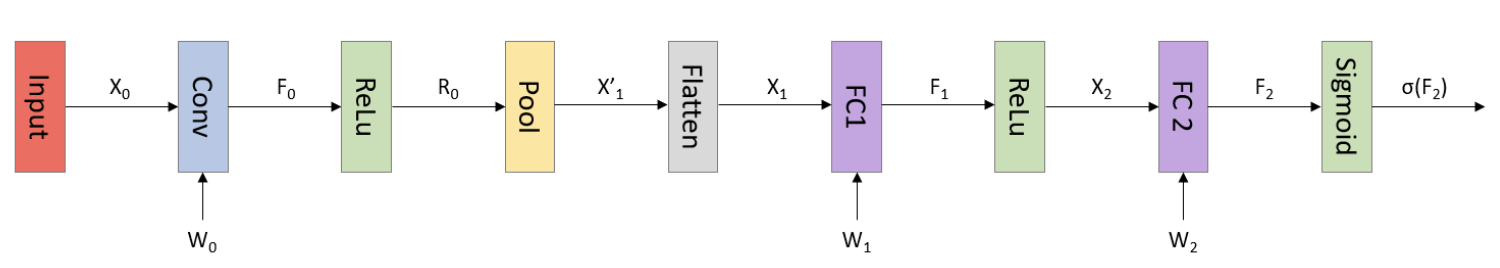
\includegraphics[width = 13cm]{mp3_1}
		\end{center}
		\caption{Architecture for MP3}
	\end{figure}

\section{Algorithm}
	\subsection*{Extract the data feature and Normalize}
	In this part, we load the image and separate them to training set and validation set. Then, we shuffle the training set by shuffle function and batchify them with the same batch size. Next, we normalize the feature in training set by dividing the value with 256 because the RGB value is between 0 to 255 to keep the pixel value in range (0, 1).
	\subsection*{Forward Propagation}
		In forward propagation part, we can calculate our lost and store some information like $R_0$ and $F_1$ and use them to update our weight in backward propagation.
		\begin{itemize}
  		\item 2D Convolution \\
			Using the following formula to calculate the 2D convolution with filter $W_0$. We initialize the $W_0$ to $N(0, 0.05^2)$. The size of $W_0$ should be $5 \times 5 \times 3$.
			$$u[n_1, n_2, j, k]*x[n1, n2, j] = \sum_j \sum_{m_1} \sum_{m_2} u[n_1-m_1, n_2-m_2, j, k]x[m_1, m_2, j]$$
			After 2-D convolution, we first change the dimension of the image from $100 \times 100$ to $96 \times 96$. Also, the channels of the output are not the channels of the input anymore although in this mp, the numbers of channels are both 3 for input and output channels.
  		\item First ReLU Layer \\
			We add the activation function (ReLU) to introduce non-linearity into the network.
			$$ReLU(x) = max(0, x)$$
			\item Max pooling \\
			In this step, we max use the maximum number in the region of max pool window, and record the chosen number in R0 mask. After the max pooling, we can reduce the size the input and the dimension become $8 \times 8 \times 3$. The formular for max pooling is
			$$X_1'[n_1, n_2, k] = \underset{(m_1, m_2) \in \mathcal{A}(n_1, n_2)}{max} max(0, R_0[m_1, m_2, k])$$
			\item Flatten Data \\
			Take a 4D array and flatten it into a 2D array. The shape of $X_1'$ is $N \times 8 \times 8 \times 3$ and after the pooling, the shape of the $X_1$ is $N \times 192$.
			\item First Fully Connected Layer \\
			In this part, we will need to derive the linear combination of input feature with filter. The size of input feature $X_1$, is $N \times 192$ where $192$ is the number of input features and filter $W_1$ is of size $ 192 \times 2$ where $2$ is the number of output fully connected nodes. After fully connected, we can reduce the dimension of the neural network.
			\item Second ReLU Layer \\
			In this part, we add the activation function to introduce non-linearity into the network. For this step, we also choose ReLU function as our activation function.
			\item Second Fully connected Layer \\
			In this part, we will need to derive the linear combination of Input feature and filter. In this part, there will be one fully connected node.
			\item Sigmoid Function \\
			In this part, we use the Sigmoid function as the activation function and introduce non-linearity in our neural network. The function of Sigmoid function is the following:
			$$\sigma(x) = \frac{1}{1+e^{-x}}$$
			\item Loss Function \\
			After we find $\sigma(F_2)$, we can calculate the lost by the following equation:
			$$L = \frac{1}{N}\sum_{i=1}^N -y_ilog(\sigma(f_{2i})) - (1-y_i)log(1-\sigma(f_{2i}))$$
		\end{itemize}

	\subsection*{Test Forward Propagation}
		After we complete the forward pass, we run the code on the $cnn\_fwd$ function with the pre-trained weights $W_0$, $W_1$ and $W_2$. The result is following figure:
		\begin{figure}[ht]
			\begin{center}
				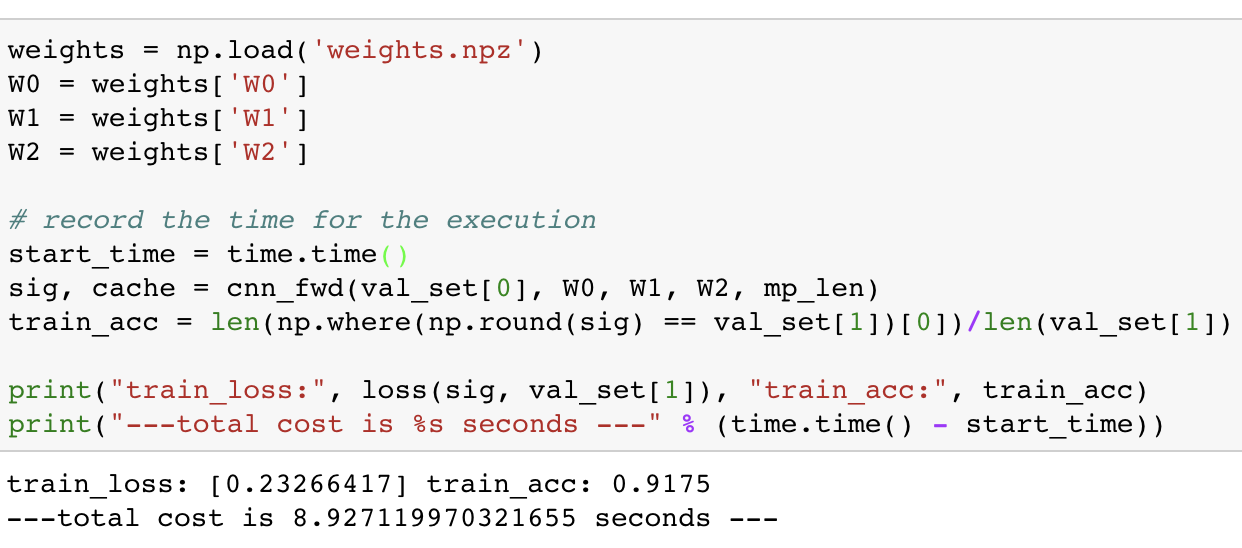
\includegraphics[width = 13cm]{forward_test}
			\end{center}
			\caption{Forward Test}
		\end{figure}

	\section*{Backward Propagation}
		In backward propagation part, we use the gradient descent algorithm to update our our weight $W_0$, $W_1$, and $W_2$.\\
		The equation for gradient descent algorithm is
		$$W_i \leftarrow W_i - \eta \frac{\partial L}{\partial W_i} \ for \ i = 0, 1, 2$$
		where $\eta$ is the learning rate of the model. We set $\eta = 0.1$ at the very beginning.\\
		In this program, we will update the W0,W1,W2 by the gradient descent algorithm in the following procedure:
		\begin{itemize}
			\item Update $W_2$ \\
			In this part, we will find the $\frac{\partial L}{\partial W_2}$ in the following substeps:
			\begin{enumerate}
				\item $\frac{\partial L}{\partial F_2} = \frac{1}{N} (\sigma(F_2) - Y)$
				\item $\frac{\partial L}{\partial W_2} = X_2^T \frac{\partial L}{\partial F_2}$
			\end{enumerate}
			\item Update $W_1$ \\
			In this part, we will find the $\frac{\partial L}{\partial W_1}$ in the following substeps:
			\begin{enumerate}
				\item $\frac{\partial L}{\partial X_2} = \frac{\partial L}{\partial F_2} W_2^T$
				\item $\frac{\partial L}{\partial F_1} = \frac{\partial L}{\partial X_2} \bigodot unitsetp(F_1)$ \\
				[0.12in]
				Notice here, the $\bigodot$ means element-wise multiplication.
				\item $\frac{\partial L}{\partial W_1} = X_1^T \frac{\partial L}{\partial F_1}$
			\end{enumerate}
			\item Update $W_0$ \\
			In this part, we will find the $\frac{\partial L}{\partial W_0}$ in the following substeps:
			\begin{enumerate}
				\item $\frac{\partial L}{\partial X_1'} = \frac{\partial L}{\partial F_1} W_1^T$
				\item $\frac{\partial L}{\partial X_1} = reshape(\frac{\partial L}{\partial X_1'})$ \\
				[0.12in]
				Since in the forward propagation, the flatten operation just reshape the size of the 2D array, we need to undo the reshape operation to get the correct size of the matrix $\frac{\partial L}{\partial X_1}$
				\item $\frac{\partial L}{\partial R_0}$ \\
				[0.12in]
				In this step, we reverse the step of max pooling by using the $R_0$ mask matrix stored in cache.
				\item $\frac{\partial L}{\partial F_0} = \frac{\partial L}{\partial R_0} \bigodot unitsetp(F_0)$
				\item $\frac{\partial L}{\partial W_0}$ \\
				[0.12in]
				At last, we get $\frac{\partial L}{\partial W_0}$ by redo the 2D convolution. The formula is:
				\begin{align}
				\frac{\partial L}{\partial W_0[m_1, m_2]} & = \sum_{n_1}\sum_{n_2} \frac{\partial L}{\partial F_0[n_1, n_2]} \frac{\partial F_0[n_1, n_2]}{\partial W_0[m_1, m_2]} \\ & = \sum_{n_1}\sum_{n_2} \frac{\partial L}{\partial F_0[n_1, n_2]} X_0[n_1-m_1, n_2-m_2]
				\end{align}
				This step can be implemented by $signal.correlate2d$ function followed by flipping the derived matrix.
			\end{enumerate}
		\end{itemize}

	\subsection*{Test Backward Propagation}
		After we complete the backward pass, we run the code on the $cnn\_bwd$ function with all weights $W_0$, $W_1$ and $W_2$ being ones. The result is following figure:
		\begin{figure}[ht]
			\begin{center}
				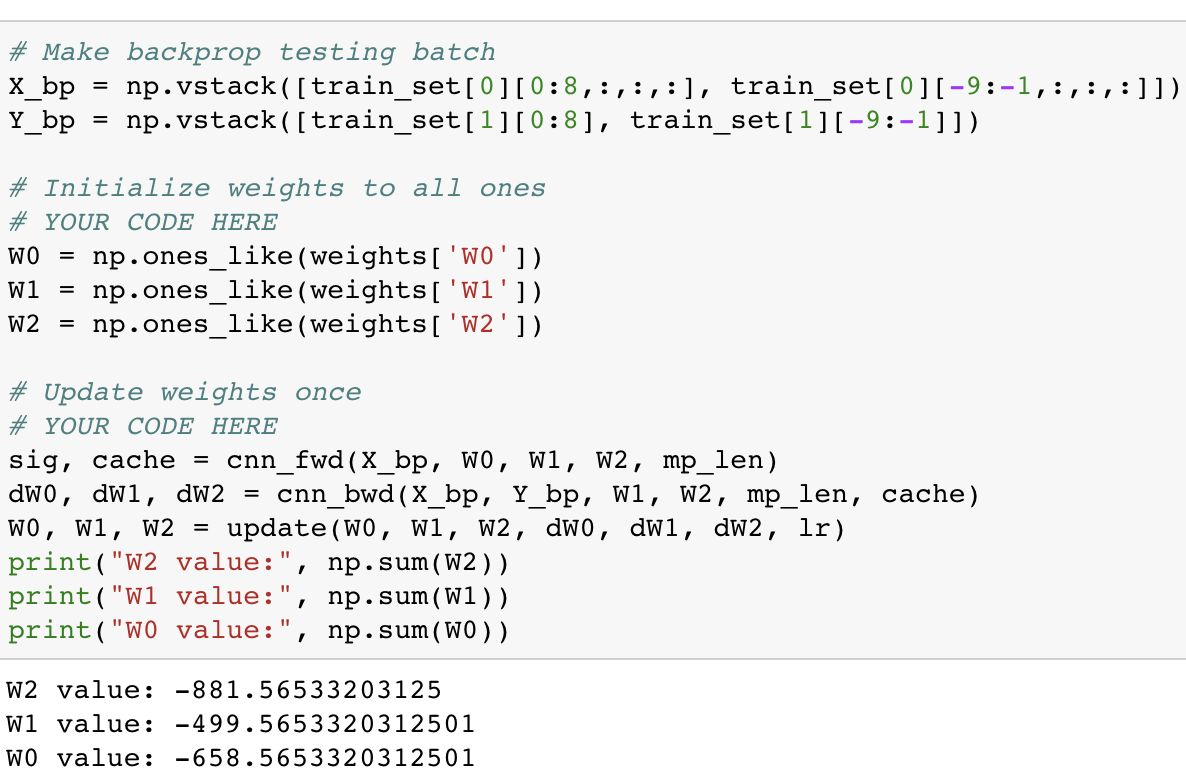
\includegraphics[width = 13cm]{back_test}
			\end{center}
			\caption{Backward Test}
		\end{figure}
		\newline
		Notice here, the results of our model have a offset of 47 compared to the given reference results. This is caused by the fact that the order of the image read by given function is different.

	\subsection*{Iteration}
		In this step, we combine the forward and backward process mentioned above and iterate for 20 epoches. After we finish one iteration, we will bachify the training data again. The reason why we need to do this is that we need to avoid overfitting. After every epoch, we record the loss and the accuracy of the model. This helps us plot the accuracy versus epoch and loss versus epoch.

	\section{Result}
		First figure is the accuracy vs epoch for the lab.
		\begin{figure}[ht]
			\begin{center}
				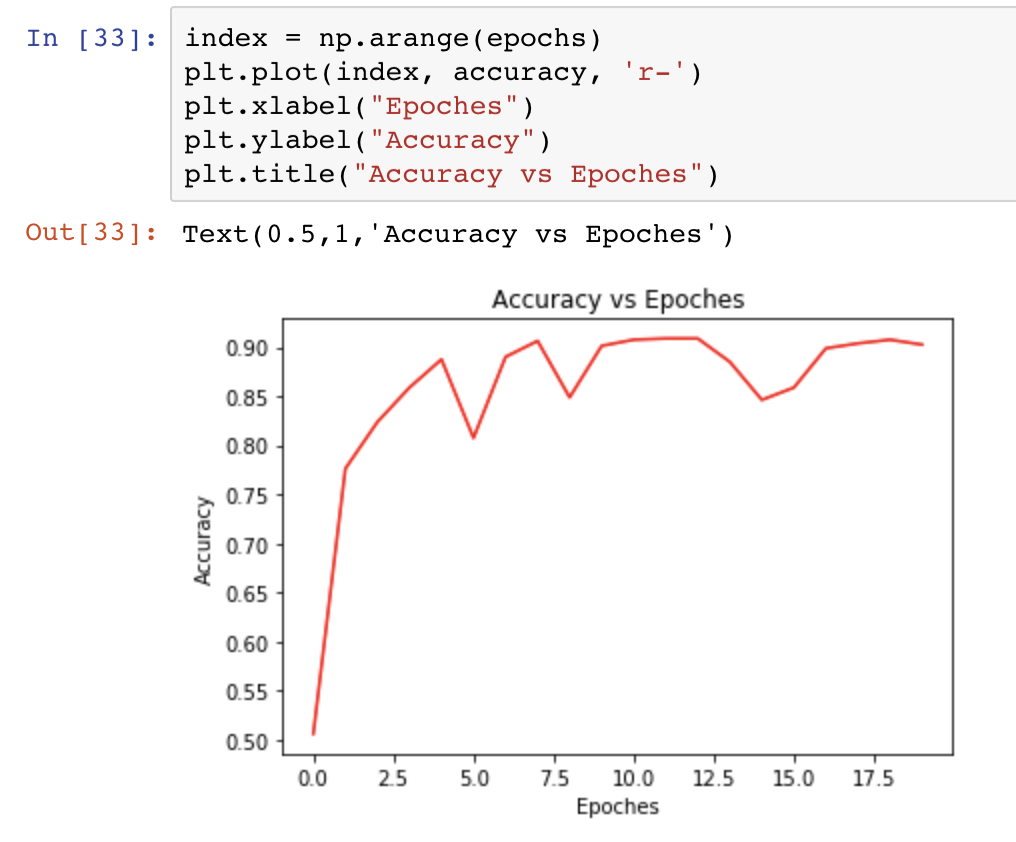
\includegraphics[width = 8cm]{acc}
			\end{center}
			\caption{Accuracy vs Epoch}
		\end{figure}
		\newline
		Second figure is the loss vs epoch for the lab.
		\begin{figure}[ht]
			\begin{center}
				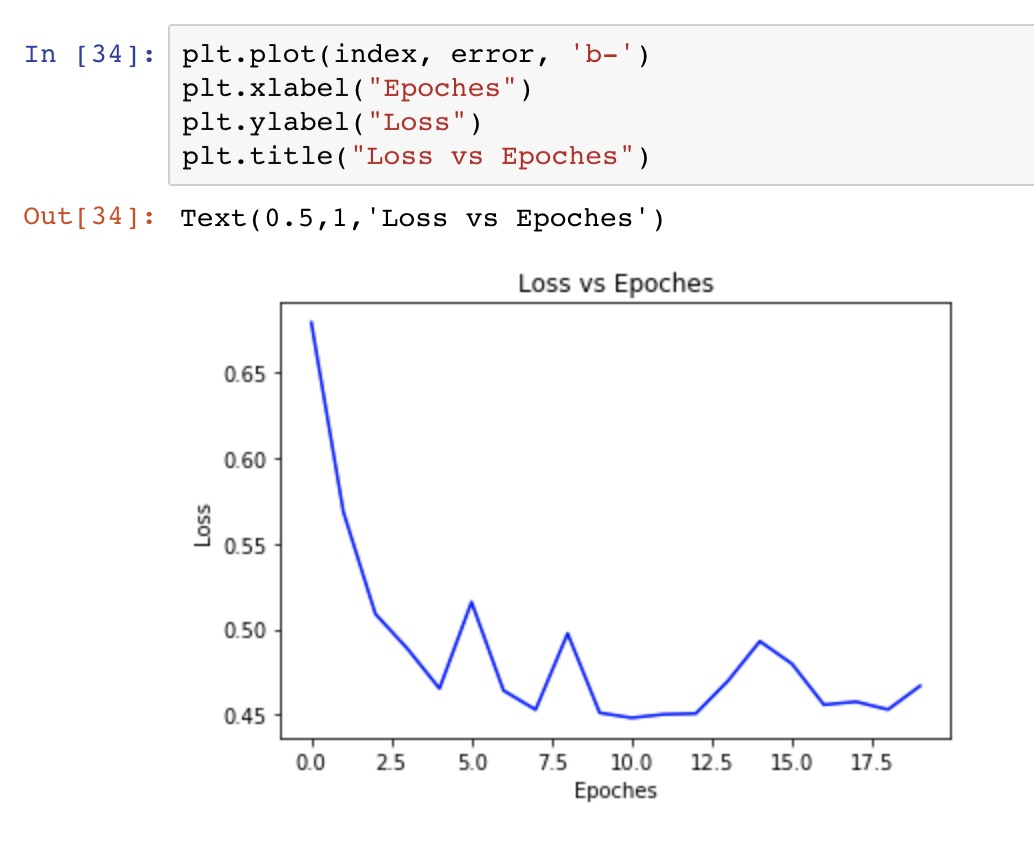
\includegraphics[width = 8cm]{loss}
			\end{center}
			\caption{Accuracy vs Epoch}
		\end{figure}
		\newline
		Following figure shows the accuracy for the trained weights on the validation set.
		\begin{figure}[ht]
			\begin{center}
				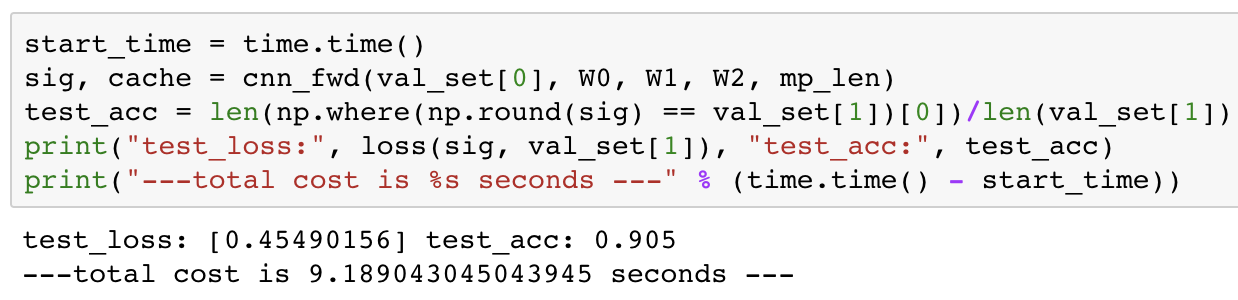
\includegraphics[width = 12cm]{acc_val}
			\end{center}
			\caption{Accuracy vs Epoch}
		\end{figure}
		\newpage
		\noindent
		Following figure gives the confusion matrix for the model.
		\begin{figure}[ht]
			\begin{center}
				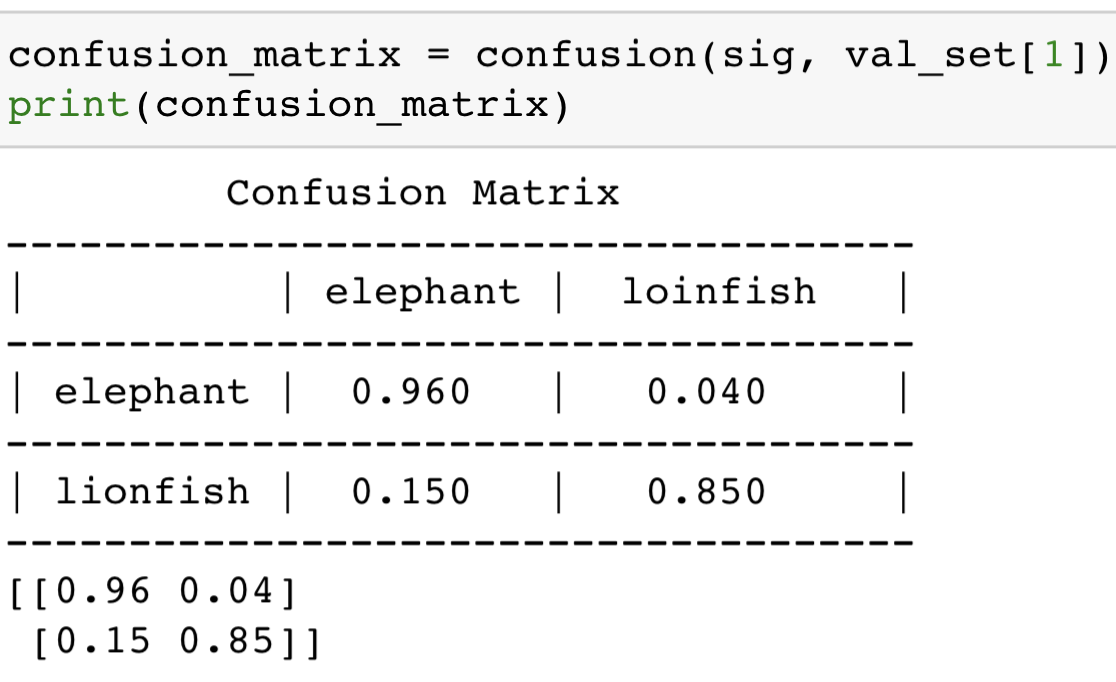
\includegraphics[width = 8cm]{confusion}
			\end{center}
			\caption{Confusion Matrix}
		\end{figure}
		\newline
		In the confusion matrix, we can see that the model is very accuracy on detecting elephant but not very well on detecting lionfish. In this next section (Analysis), we can see that why lionfish is harder to recognize.\\
		Following figure gives the result of the image after applying the convolution.
		\begin{figure}[ht]
			\begin{center}
				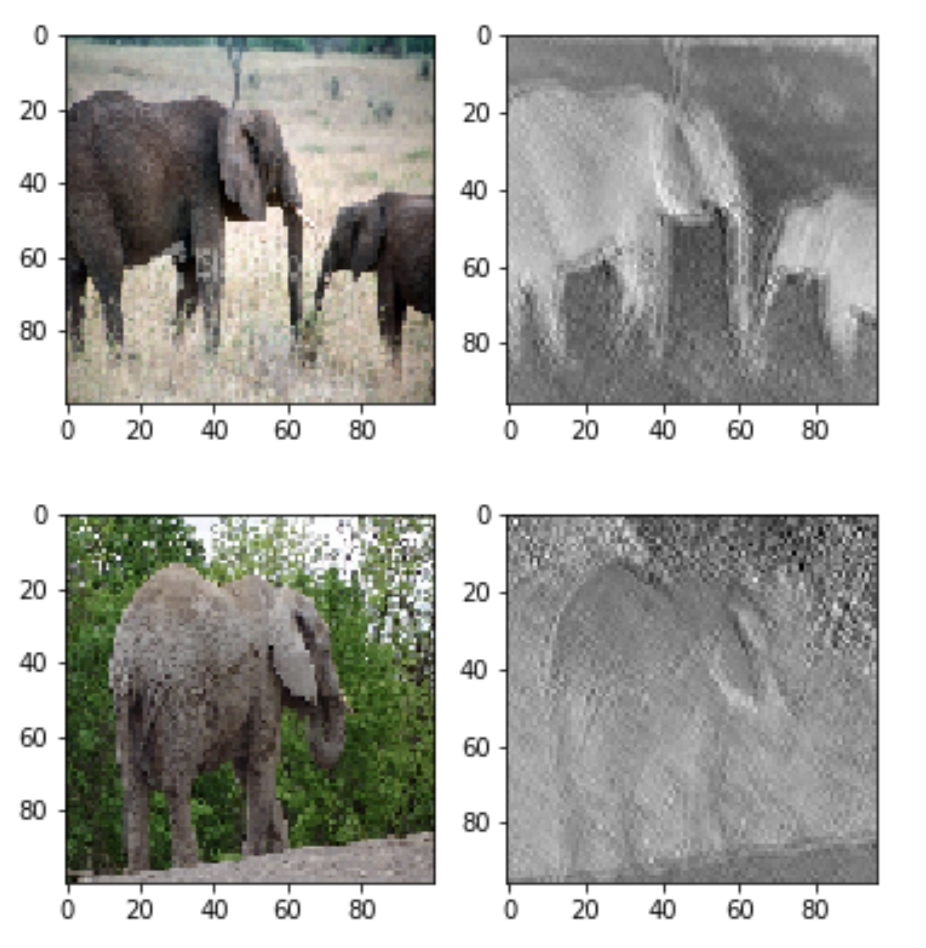
\includegraphics[width = 6cm]{elephant}
			\end{center}
			\caption{Elephant Image}
		\end{figure}
		\begin{figure}[ht]
			\begin{center}
				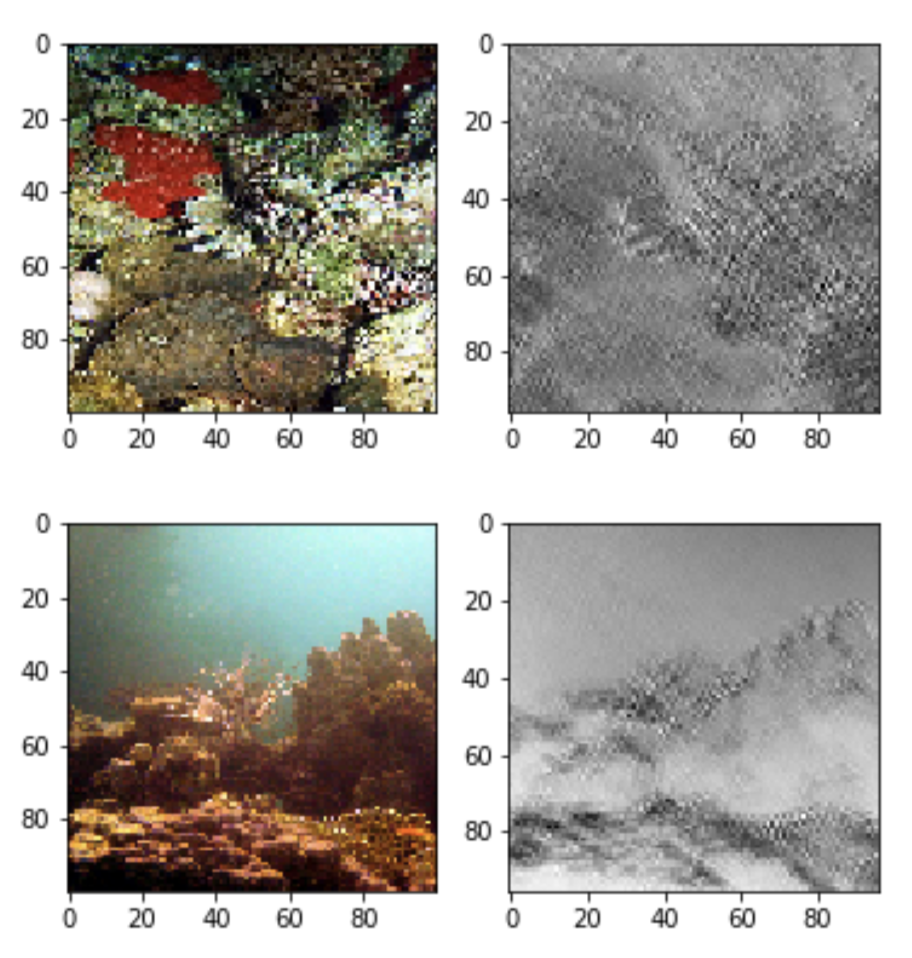
\includegraphics[width = 6cm]{lionfish}
			\end{center}
			\caption{Lionfish Image}
		\end{figure}

	\section{Analysis}
	\begin{itemize}
		\item Normalize Data\\
		When we extract data, we should normalize them by divide data by 256. The reason why we need to normalize the data is that when we process the training, we first use the input data to do the forward pass and then use the gradient descent to update the weights. We update the weights by subtracting the product of the learning rate and gradient of loss from previous weights. If we do not normalize the input data, then if two features have different range (for example, one is 200 and the other is around 10), then the update of the weights will have totally different influence on these features. Therefore, we want to normalize the input to the same scale as the learning rate.
		\item Plot of Accuracy vs Epoch \\
		At the first 4 epoches, our accuracy increases fast due to the learning procoess of the model. We also notice that the accuracy sometimes decrease significantly. We think the reason why it decreases is that the learning rate is too large in that epoch. In the previous epoch, the weights are closed the local optimal value, and after one iteration, the weights are updated but miss the optimal value because learning rate is relatively large compared to the gap between the current weights and the optimal weights. But this does not often happen and at last, the accuacy converges to approximate 90\%. To fix the problem that the accuracy might bounce up and down, we add a decay in learning rate, which helps the accuacy converge. This process is described in Extra Credit part.
		\item Convolve Input Images with Trained Weights \\
		In this experiment, we convolve the input image with trained weights $W_0$ and the graph is shown above. We find that after convolution, we can generate the outline of the input image and we believe that after the convolution, it learned the outline of the input image.
		\item Comment on the Classification \\
		After we test the accuracy, we find that the lionfish class is confused most and the reason is that the color of lionfish is closer to the environment than element’s so that after convolving with the filter, the outline is not clear and therefore the model declare a wrong label. The feature that confuse the model is color because after we check the picture that produce the wrong label, we find that in these pictures, the color of lionfish is close to the color of coral around it and the outline is not clear after convolution with $W_0$. \\
		The second reason is that the picture itself is blurry just like the third picture above and we even cannot distinguish what it is by our eyes.

	\end{itemize}
	\section{Extra Credit}
	\subsection{Data Argumentation}
	\begin{itemize}
		\item Introducion \\
		In this part, we use the data argumentation to generate more training data to feed in the model and finally make the model have a higher accuracy on the test of validation set.
		\item Algorithm \\
		For every input image, we generate a new image by rotation, scaling, shifting and interpolation. For an input image $I(u, v)$, we generate the output image $J[x, y]$. Notice here the parenthesis () used in input image and square brackets [] used in output image. The goal of data argumentation is to generate new image with the same size (here a $100\times100\times3$ 3D array). Usually if the output coordinates $x$, $y$ are integers, the correspond input coordinates $u$, $v$ are not integers and therefore we need to interpolate. To perform the transformation of the image, we do the transformation of the coordinates.
		\item Coordinates Transform \\
	  Let $\vec{u} = \begin{bmatrix}
	           u \\
	           v \\
	           1
	         \end{bmatrix}$
	  and $\vec{x} = \begin{bmatrix}
	           x \\
	           y \\
	           1
	         \end{bmatrix}$,
	  then we can wrtie the transformation of the coordinates as the matrix-vector multiplication as following:
	  $$\vec{u} = T\vec{x}$$
	  where $T$ is the transformation matrix. We can find the pixel of the output image at [$x$, $y$] as the pixel of the input image at ($u$, $v$). In our implementation, we have three kinds of transformation. The first is rotation. This can be captured by a matrix $T_1 = \begin{pmatrix}
	                cos(\theta) & sin(\theta) & 0 \\
	                -sin(\theta) & cos(\theta) & 0 \\
	                0 & 0 & 1
	               \end{pmatrix}$, and we set $\theta = \frac{\pi}{6}$ to rotate 30 degrees.
	  Our second transformation is scaling. The matrix corresponding to this is $T_2 = \begin{pmatrix}
	                1 & 0 & 0 \\
	                0 & \frac{2}{3} & 0 \\
	                0 & 0 & 1
	               \end{pmatrix}$, which scale the horizontal axis by $\frac{2}{3}$.
	  At last, we shift the output image to the left by 10 pixels by applying the last matrix. $T_3 = \begin{pmatrix}
	                1 & 0 & 0 \\
	                0 & 1 & 10 \\
	                0 & 0 & 1
	               \end{pmatrix}$.
	  Therefore, the relations between input coordinates and output coordinates are
	  $$\vec{u} = T_3T_2T_1\vec{x}$$

		\item Interpolation \\
		As mentioned above, we need to do the interpolatioin since we do not have the pixel value at ($u$, $v$) in input image. We use the linear interpolation which find the pixel value at ($u$, $v$) by linearly combine the nearest four pixels around point ($u$, $v$). The interpolation formular is given by
	  $$I(u, v) = \sum_m \sum_n I[m, n]h(u-m, v-n)$$
	  For linear interpolation, the filter $h$ is given by
	  $$h(u, v) = max\{0, (1-|u|)(1-|v|)\}$$
	  With the linear interpolation, the summation above to derive $I(u, v)$ can be written as the sum of following 4 terms (suppose $m = \lfloor u\rfloor$, $n = \lfloor v\rfloor$, $e = u - m$ and $f = v - m$)
		\begin{dmath}
	  I(u, v) = (1-e)(1-f)I[m,n] + (1-e)fI[m, n+1] + e(1-f)I[m+1, n]+efI[m+1, n+1]
		\end{dmath}
		\item Result \\
		After applying the data argumentation of the training set, the size of the training set increases from 2000 to 4000 and the plot for accuracy and loss are following figures.
		\begin{figure}[ht]
			\begin{center}
				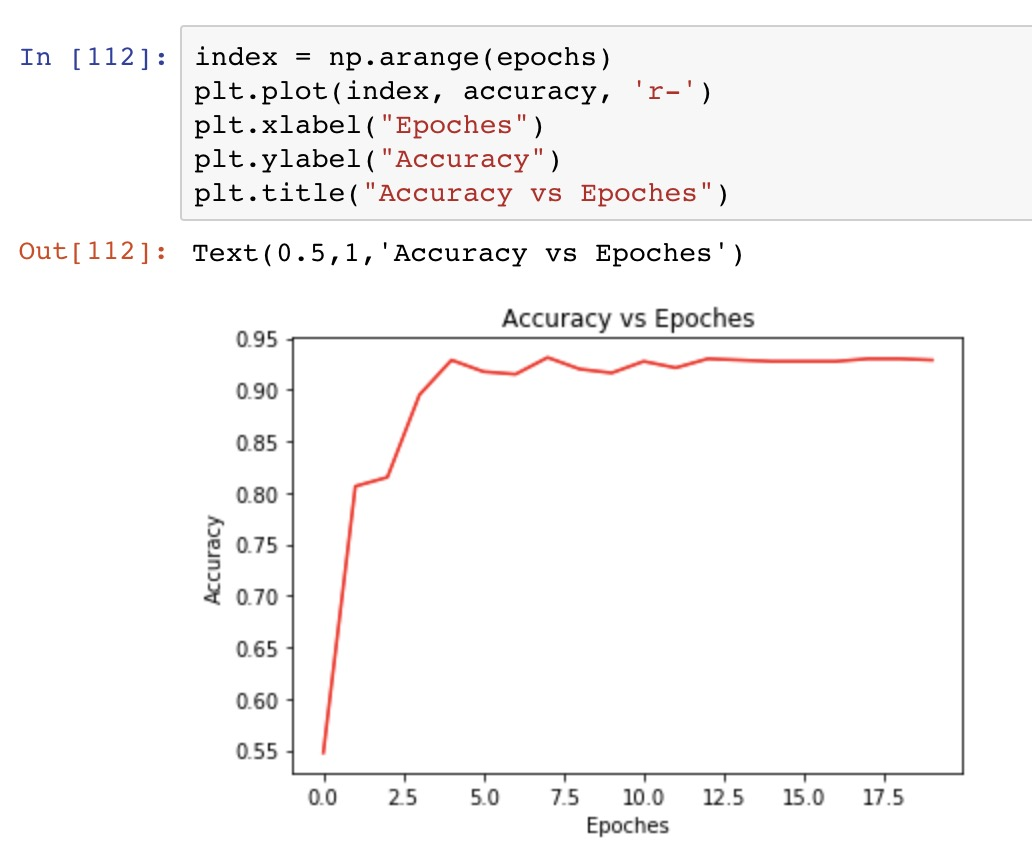
\includegraphics[width = 10cm]{da_acc}
			\end{center}
			\caption{Accuracy vs Epoch}
		\end{figure}
		\begin{figure}[!h]
			\begin{center}
				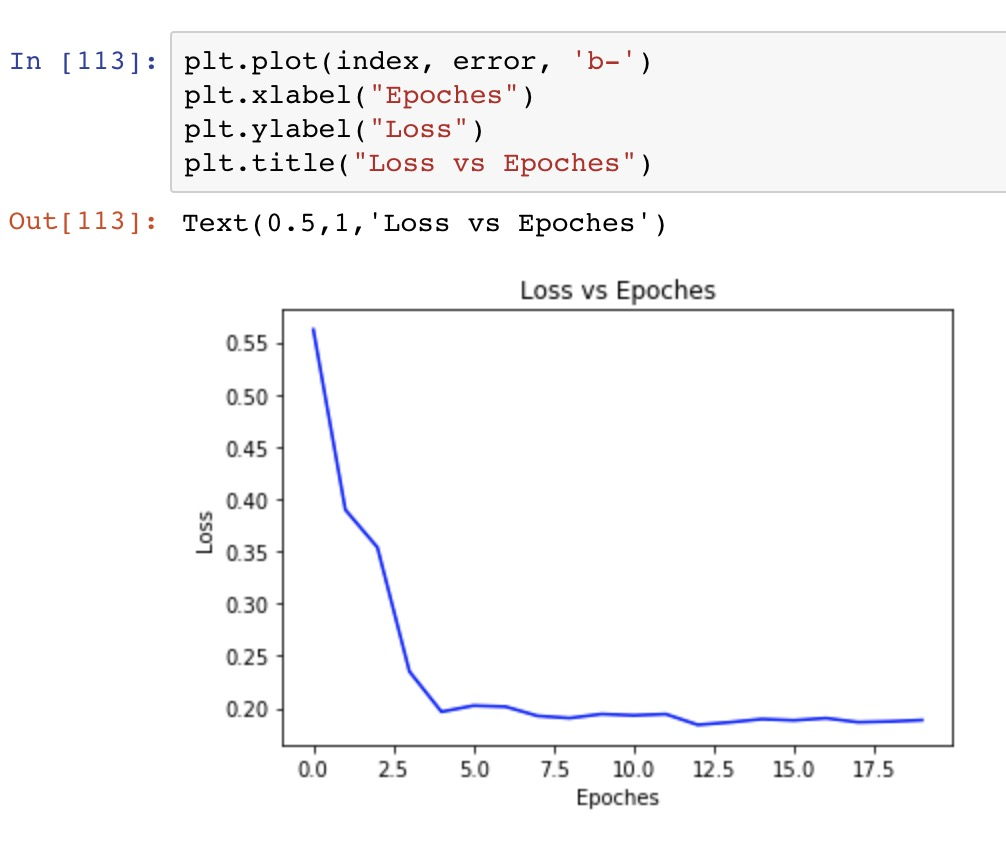
\includegraphics[width = 10cm]{da_loss}
			\end{center}
			\caption{Loss vs Epoch}
		\end{figure}
		\newpage
		From the plot, we can see that the accuracy increasees to roughly 93\% compared to the roughly 90\% when not applying the data argumentation.
		\end{itemize}

	\subsection{Gradient Descent Decay}
	As mentioned above, if not applying the decay in learning rate, the accuracy of the model sometimes bounce significant between 80\% and 90\%. Therefore, we decide to decrease the learning rate while the training is processing. We set a decay of 0.5 when accuracy exceed 90\%. This means that if the accuracy is greater than 0.9, the learning rate for next epoch will be halved compared to this epoch. In this way, the accuracy will become more smooth than before and the result is shown in the following figure.
	\begin{figure}[ht]
		\begin{center}
			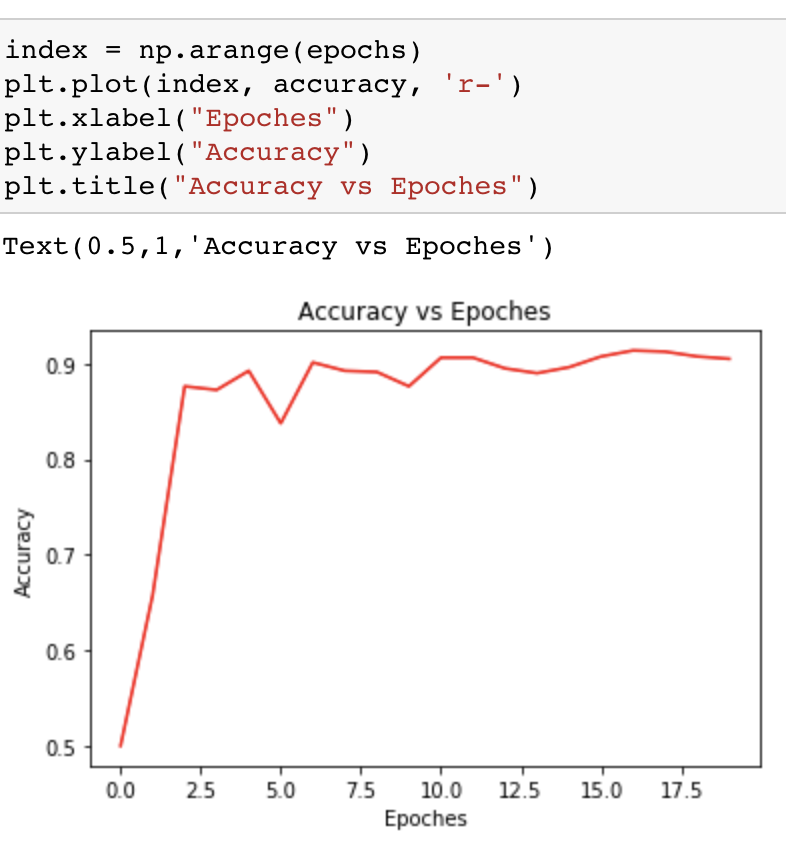
\includegraphics[width = 6cm]{decay_acc}
		\end{center}
		\caption{Accuracy vs Epoch}
	\end{figure}
	\begin{figure}[!h]
		\begin{center}
			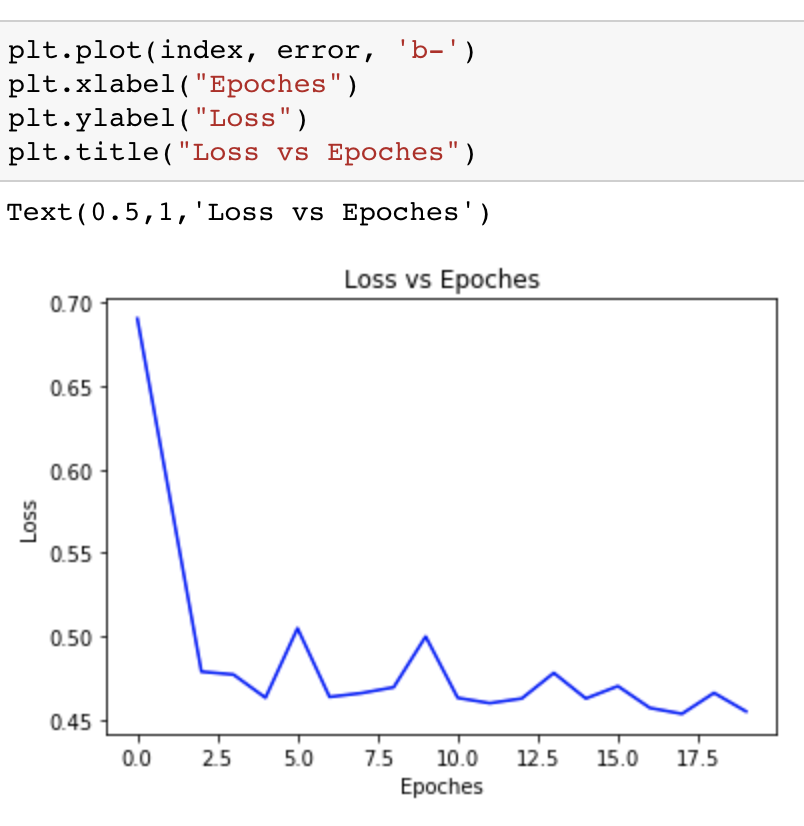
\includegraphics[width = 6cm]{decay_loss}
		\end{center}
		\caption{Loss vs Epoch}
	\end{figure}


\end{document}
